\setstretch{1.5}
\chapter{Experimental Apparatus}

\tab A major portion of the research presented in this dissertation has been experimental in nature. All of the plasma and etch experiments were performed using an Applied Materials Precision Etch 8300 (AME-8300)\footnote{The system was not truly an 8300 series etcher, but instead a hybrid between the 8100 and 8300 series. It is affectionately referred to as the “Mule.”} which was donated by the manufacturer to the SolidState Electronics Laboratory (SSEL) at the University of Michigan in 1987. This etcher, as with most commercially available etch systems, was designed for a production environment and was not configured for in situ measurements or the application of real-time control techniques. The first portion of my research focused on modifying our AME-8300 for the implementation of real-time feedback control.

\setstretch{.75}
\section{Precision Etch 8300 Hexode RIE}

\setstretch{1.5}
\tab The AME-8300 is a hexode reactive ion etcher (see Figure 2.1), where wafers are placed vertically on a hexagonally shaped powered electrode and the bell jar acts as the grounded electrode. The AME-8300 at the University of Michigan was designed to simultaneously etch 18 four inch wafers, though in this research it was used as a single wafer etcher. The hexode


\setstretch{.75}
\begin{figure}[H]
	\centering
	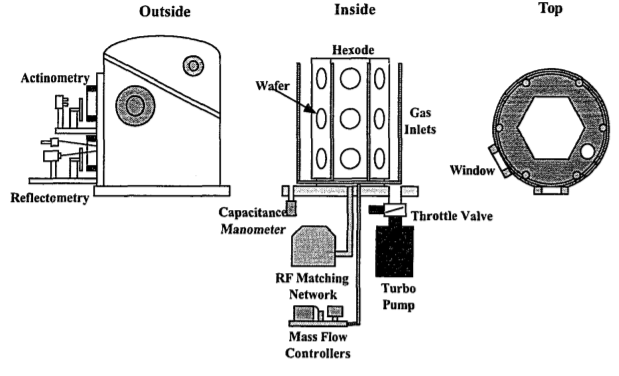
\includegraphics[scale = .6]{Figure 2.1}
	\bf\caption{ Precision Etch 8300 hexode reactive ion etcher.}
	\label{fig:2.1}
\end{figure}

\setstretch{1.5}
\noindent has approximately one third the surface area of the bell jar. As was seen in Equation 1.7, this difference in surface area allows high energy ion bombardment of the powered electrode while minimizing the bombardment of the grounded electrode and other chamber surfaces. Process gases are mixed in a manifold and then enter the chamber in a sprinkler fashion through vertical pipes across from each corner of the hexode. The gas reactants are
removed from the chamber by a turbomolecular pump with the exhaust conductance from the chamber regulated by a throttle valve. It is important to note that our system does not
have a load lock, thus requiring the chamber to be vented to atmosphere each time a wafer is loaded. As will be explained in Section 4.2.1, this has had a strong impact on the etching
process.

The AME-8300 comes standard with two viewports at which optical sensors can be mounted. One of the viewports is on the upper portion of the clam shell and moves with the top of the chamber when wafers are loaded. The other port has occasionally beenoccupied by an infrared camera and more recently by a mass spectrometer. Neither port provided a stable mounting point for the optical sensors used in this research. Therefore, two additional 4 inch optical viewports were added to the face of the reactor where the gate valve for a load lock would have been situated. Optical breadboards were mounted below each of these windows to create a flexible and sturdy platform for the optical sensors.


\subsection{Actuators}

\tab It was necessary to upgrade some of the actuators on the reactive ion etcher in order
to improve our ability to control the process. The existing throttle valve, which regulates
the exhaust of reactant gases from the chamber, had several shortcomings from the point
of view of dynamic control. These included a large leakage conductance when fully closed,
an operating regime near saturation, hysteresis in the motion of the valve, and the lack of
a sensor for measuring actual valve position. The valve was replaced with an MKS Type
652A Throttle Valve and an MKS Type 653 Throttle Valve Controller. This valve was sized
to be smaller than the old one, thus moving the operating region away from saturation. In
addition, the valve has a low leakage conductance when fully closed, a good response time,
and a sensor to measure the actual valve position. The throttle valve controller allows
either the specification of a pressure setpoint to be regulated by an internal PID loop or
the direct control of throttle position. The RF power actuator includes a Henry Electronics
2000W, 13.56 MHz generation unit and an RF Services RF8300RL matching network. The
AME-8300 was originally supplied with a Micro-Match 8300N matching network supplied by
Applied Materials. The upgraded matching network does a better job matching impedances
(as measured by reflected power), has a quicker response time, and has a peak-to-peak
voltage ($\text{V}_{pp}$) measurement. The $\text{V}_{pp}$ is used by related research efforts, but not utilized in this work. Gas flows are regulated by MKS Type 2259C Mass Flow Controllers and are mixed in a manifold prior to entering the process chamber. These flow controllers were sized to give the highest resolution over the flow rates necessary for this work.

During this research, short intermittent fluctuations in the gas flow rates were noted.
It was suspected that these were due to the pressure regulator on the gas bottles [36].
These fluctuations, while short enough to have negligible effect on etch results, could make
dynamic modeling difficult. The fluctuation problem was solved by placing a 2 $\mu m$ VCR
filter gasket in the outlet valve just downstream of the pressure regulator.

\subsection{Sensors}

\tab Three types of sensors were used to make in situ measurements of the plasma environment for feedback control. The dc bias voltage ($\text{V}_{bias}$) was measured through an inductive
tap on the powered electrode side of the matching network. Pressure in the chamber was
monitored by an MKS Type 127A Baratron Capacitance Manometer. A typical operating
regime for reactive ion etching in the AME-8300 is around 20 mTorr. The manometer, which
originally had full scale range of 1 Torr, was resized to 100 mTorr to improve its resolution.
The fluorine concentration is estimated via optical emission spectroscopy using actinometry; details of actinometry are presented in Section 2.1.3. In addition to these sensors, the
AME-8300 was fitted with a laser reflectometry system to measure in \textit{situ} etch rate; details on the reflectometry system are presented in Section 2.1.4. This measurement was only
used to verify the performance of the control schemes and not for real-time feedback.

\subsection{Fluorin Concentration Estimate}

\tab The fluorine concentration in the bulk plasma is strongly related to properties of the
etch [44]. Unfortunately, it is not possible to directly measure fluorine concentration without
perturbing the plasma. In research, various probes are sometimes used to sample the plasma
chemistry; it is very difficult to relate plasma characteristics near the probe to those of the
unperturbed plasma [56]. These probes are therefore not useful in measuring properties of
a plasma during processing. Instead, the fluorine concentration is indirectly measured via
optical emission spectroscopy using a technique known as actinometry.

\setstretch{1.75}
\noindent\large\bf Actinometry

\normalsize\normalfont The emission intensity from a spectral line of species x is given by [58]

\setstretch{1}
\begin{align}
	I_{x} &= N_{x} \left[ \int_{0}^{\infty} Q_{x}\left( P,N_e \right) \sigma_{x} \left( \epsilon \right) N_{e} d\epsilon   \right],
\end{align}



\setstretch{1.5}

\noindent where $N_{x}$ is the concentration of species $x$, $Q_{x}$ is the quantum yield from a given higher energy excited state to a given lower energy excited state, P is pressure, $\sigma_{x}$ is the excitation cross section from the ground state to a given excited state of electron energy $\epsilon$, and $N_{e}$ is the electron density in an electron energy range $d_{\epsilon}$. Because several of these parameters are unknown and impossible to measure, we use a technique known as actinometry [22]. In actinometry, a small amount of an inert gas, having excitation characteristics similar to the species of interest, is added to the feed gas; the inert gas is referred to as an actinometer. As will be seen below, the appropriate choice of spectral lines allows the concentration $N_{x}$ to be determined without calculating the integral in Equation 2.1. Argon is used as an actinometer for fluorine concentration estimates.

The fluorine concentration estimate is found by first noting that the spectral line intensities are proportional to the corresponding excited state population densities ($N_{x}^{*}$) of each of the species,

\setstretch{1}
\begin{align}
	I_{F} \alpha N_{F}^{*}
\end{align}

\noindent and

\begin{align}
	I_{Ar} \alpha N_{Ar}^{*}.
\end{align}

\setstretch{1.5}

\noindent It is necessary that the excitation efficiencies for the excited states corresponding to the spectral lines used in actinometry have similar dependence on plasma parameters [22]. In practice, both excited states need to have similar excitation thresholds and must only be populated from the ground state by electron collisions.

For fluorine actinometry, the 703.75 nm and 750.39 nm emission lines of fluorine and
argon, respectively, satisfy these requirements. The excited states for these transitions have
similar excitation thresholds [99], as shown in Figure 2.2. For low density plasmas, such
as those used in RIE, these states are also only populated by electron excitation from the
ground state [40]. From this choice of spectral lines:


\setstretch{0.75}
\begin{align}
	\frac{N_{F}^{*}}{N_{F}} = \frac{N_{Ar}^{*}}{N_{Ar}}.
\end{align}

\noindent Therefore, 

\begin{align}
	N_{F} = k\frac{I_{F}}{I_{Ar}}N_{Ar},
\end{align}

\setstretch{1.5}

\noindent where k is a proportionality constant known as the actinometric constant. We define $\gamma$ to be the fraction of Ar in the chamber,

\setstretch{.75}
\begin{align}
	\gamma = \frac{P_{Ar}}{P} = \frac{N_{Ar}}{N},
\end{align}

\setstretch{1.5}
\noindent where $N$ is the total concentration of species in the chamber. Note that from the ideal gas law


\setstretch{1}

\begin{align}
	N = \frac{n}{V} = \frac{P}{RT},
\end{align}

\setstretch{1.5}
\begin{figure}[H]
	\centering
	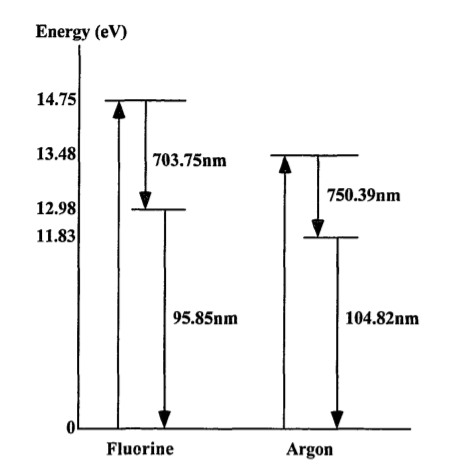
\includegraphics[scale = 1]{Figure 2.2}
	\bf\caption{ Atomic energy levels and emission wavelengths for F and Ar atoms [99].}
	\label{fig:2.2}
\end{figure}

\noindent where n is number of molecules, $V$ is the chamber volume, $P$ is the chamber pressure, $R$ is the universal gas constant ($R = 8.314 \text{J/mol } ^{\circ} K$) and T is the temperature in degrees Kelvin. Therefore,

\setstretch{1}
\begin{align}
	N_{Ar} = \gamma \frac{P}{RT}
\end{align}

\noindent and

\begin{align}
	N_{F} = k\frac{I_{F}}{I_{Ar}}\gamma \frac{P}{RT}.
\end{align}

\setstretch{1.5}

\noindent Implicit in these equations is the assumption that the neutral temperature in the plasma remains constant. This assumption is based on the fact that the radicals remain “cold” in the plasma.

In general, it is assumed that the fraction of argon in the plasma is equal to the percentage of argon in the feed gas. This assumption is reasonable as the dissociation of the feed
gases is usually between 0.01 and 10 percent [68]. This leads to the traditional estimate of
fluorine concentration

\setstretch{1}
\begin{align}
	N_{F} = \bar{k} \frac{I_{F}}{I_{Ar}}\gamma_{flw} P,
\end{align}

\setstretch{1.5}
\noindent where $\bar{k} =\frac{k}{RT}$ and $\gamma_{flw}$ is the percentage of total flow which is argon $\left( \gamma_{flw} = \frac{FLOW_{Ar}}{FLOW_{Total}} \right)$. Thus, $\gamma_{flw}$ $P$ is an estimate of the argon partial pressure ($P_{Ar}$). This equation is different from those traditionally seen in the literature [88] as it accounts for variations in the percentage of argon in the feed gas.

Throughout this dissertation no attempt was made to determine the actinometry constant $k$. In addition, during the etch rate control portion of this research the percentage of
argon in the feed gas was held constant at 5\% by premixing it with $\text{CF}_{4}$ in the gas bottle. Thus, the fluorine concentration estimate used in Chapters 3 and 4 was

\setstretch{1}

\begin{align}
	[F]= \frac{I_{F}}{I_{Ar}}P.
\end{align}

\setstretch{1.5}

In the sidewall profile control experiments, $\text{O}_{2}$ was added to the $\text{CF}_{4}$ chemistry. Initially, to insure a constant percentage of argon in the feed gas, a separate mass flow controller was used to regulate argon flow. The argon flow rate was typically quite small (~ 1.5 seem) and the exact flow rate was not very reproducible. Therefore, the premixed $\text{CF}_{4}$ /Ar bottle was again used and the percentage of argon in the gas mixture dynamically calculated. Due to this, the fluorine concentration estimate used in Chapter 5 was


\setstretch{1}

\begin{align}
	[F]= \frac{I_{F}}{I_{Ar}}\gamma_{flw}P.
\end{align}

\setstretch{1.5}

The fluorine estimator presented in Equation 2.10 assumes that the relative concentration of argon in the chamber is equal to the percentage of argon in the feed gas. In the case
when the dissociation is not negligible Equation 2.10 overestimates the actual fluorine concentration. In addition, as shown in Figure 2.3, outgassing from the chamber walls serves
to dilute the argon partial pressure. This is particularly a problem for the reactor used in
this research, as it does not have a load lock. It was necessary to expose the chamber to
the ambient atmosphere every time a wafer was loaded to be etched. In doing this, water
vapor adsorbs on the walls of the chamber; this moisture then desorbs when the plasma is
struck. Because of the large surface area of the chamber walls, the moisture causes a large
disturbance to the plasma which decays with a time constant on the order of 300 seconds.
The effect of this disturbance on the etching process will be discussed in Section 4.2.

One solution to the problems associated with dilution of the actinometer is to measure
the actual argon partial pressure in the chamber. This has been done by Jenq, \textit{et al.} ,
for both RIE and electron cyclotron resonance (ECR) plasma using a mass spectrometer
[58]. They noted that ion concentration was independent of applied power in RIE; this was
not the case for ECR plasmas. This fact supports the assumption that there is a small
percentage of dissociation in the plasma. Though not used in this research, an Extrel MS


\setstretch{1}
\begin{figure}[H]
	\centering
	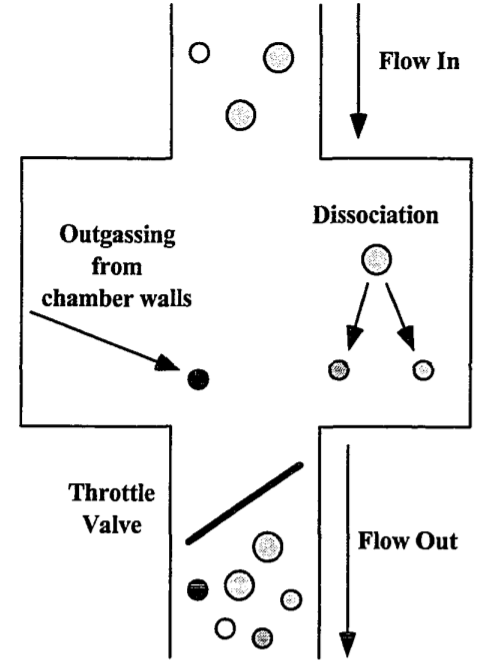
\includegraphics[scale = .5]{Figure 2.3}
	\bf\caption{ Dilution of actinometer.}
	\label{fig:2.3}
\end{figure}

\setstretch{1.5}

\noindent 250 mass spectrometer has recently been added to our AME-8300. It is our hope that this will allow us to account for argon dilution caused by outgassing from the chamber walls.


\setstretch{1.75}
\noindent\large\bf Optical Emission Hardware

\normalsize\normalfont The optics for collecting plasma emissions have gone through several iterations over the time period of this work, with the goal of providing better day-to-day repeatability and accuracy of the optical measurements. In the discussion below, I will only present the current system configuration.

The actinometry system is shown in Figure 2.4. Optical emission from the plasma is
modulated to 1 kHz using a mechanical chopper and is collected by a fused silica fiber
bundle. This bundle is bifurcated and sent to two Spex 500M 1 /2 meter monochromators,
each with a 1200 grooves/mm holographic grating with blaze wavelength of 750 nm. The


\setstretch{1}
\begin{figure}[H]
	\centering
	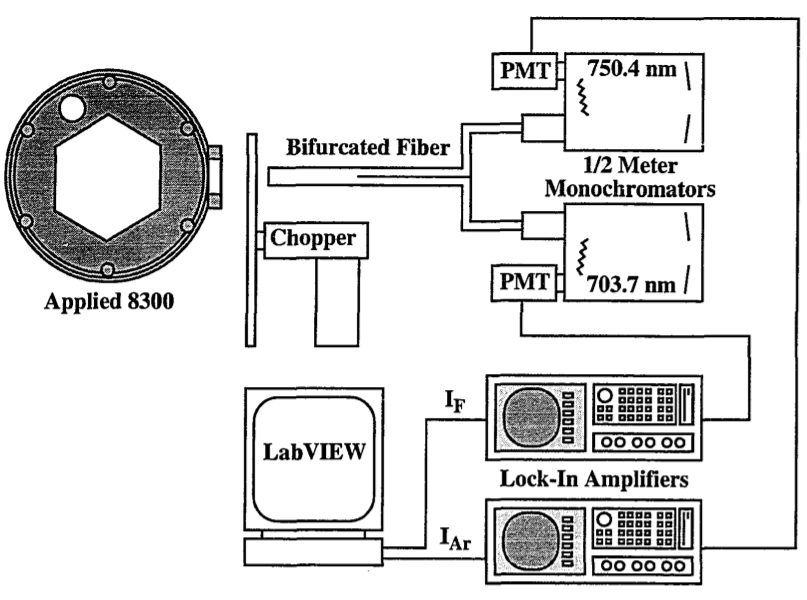
\includegraphics[scale = .5]{Figure 2.4}
	\bf\caption{ Actinometry system.}
	\label{fig:2.4}
\end{figure}

\setstretch{1.5}

\noindent monochromators are calibrated using micro-stepper motors to the 703.7 nm and 750.4 nm
wavelengths of the fluorine and argon spectra, respectively. The light is converted into
electrical signals using thermoelectrically cooled Hamamatsu R928 photomultiplier tubes
and demodulated with Stanford Research SR850 DSP Lock-In Amplifiers with a low pass
filter time constant of 30 ms. These amplifiers use automatic phase correction, thus reducing
sensitivity to chopper variations due to rf interference [9]. This system can also be used in
a scanning mode to find the optical spectrum of the plasma. Figure 2.5 shows the optical
spectrum between 675 and 775 nm for a $\text{CF}_{4}$/Ar plasma.

\setstretch{1}
\begin{figure}[H]
	\centering
	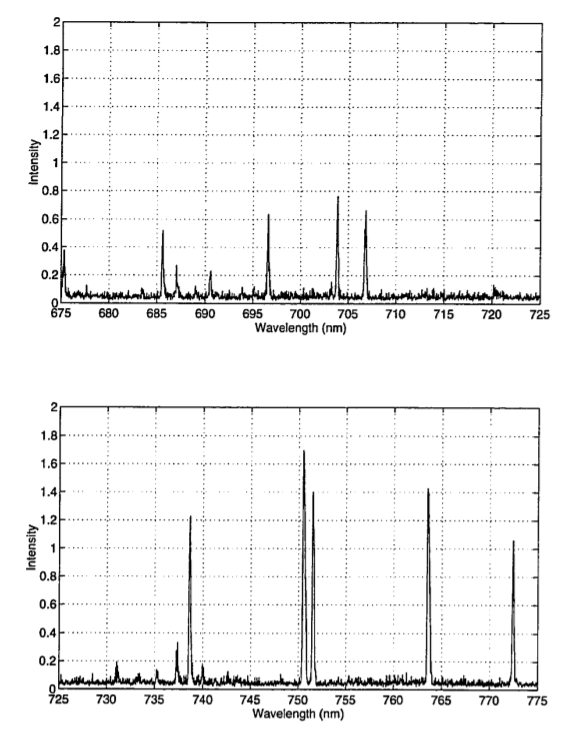
\includegraphics[scale = .8]{Figure 2.5}
	\bf\caption{ Optical spectrum of a $\text{CF}_{4}$ / Ar plasma.}
	\label{fig:2.5}
\end{figure}

\setstretch{1.5}

\subsection{Etch Rate Measurement}

\tab One of the performance metrics used for evaluating the effectiveness of the control
strategies was their the ability to reject disturbances to etch rate. In order to make this
evaluation, the etch rate was measured during the length of the run through optical interferometry. After presenting a brief overview of interference from thin films, the hardware
used in this research will be presented.

\setstretch{1.5}
\noindent\large\bf Interference in thin films

\setstretch{1.5}

\normalsize\normalfont Due to optical interference, a stack of thin film layers exhibits a reflectance that is dependent on the wavelength of the incident light and the thicknesses of each film layer. This is seen by first noting that the change in phase of light traversing the $m$th layer of film is given by


\setstretch{.5}
\begin{align}
	\delta_{m} = \frac{2\pi}{\lambda_{0}}n_{m}d_{m}\text{cos}\psi_{m},
\end{align}

\setstretch{1.5}

\noindent where $\lambda_{0}$ is the wavelength of the light in a vacuum, is the index of refraction of layer $m$, $d_{m}$ is the thickness of layer $m$, and $\psi_{m}$ is the angle at which the light is incident on the interface between layers $m$ — 1 and $m$. For light at normal incidence, the Fresnel reflection and transmission coefficients for an interface between films $m$ - 1 and $m$ are given by [49]


\setstretch{.4}

\begin{align}
	r_{m} = \frac{n_{m-1}-n_{m}}{n_{m-1}+n_{m}}
\end{align}

\noindent and

\begin{align}
	t_{m} = \frac{2n_{m-1}}{n_{m-1}+n_{m}},
\end{align}

\setstretch{1.5}
\noindent respectively. For light at angles other than $\psi_{m}=0$ see [50].

We consider the stack of $k$ thin film layers on a thick substrate (as shown in Figure 2 .6 )
and adopt the convention that $E_{m}^{+}$ is the electric field traveling down at interface $m$ and $E_{m}^{-}$ 


\begin{figure}[H]
	\centering
	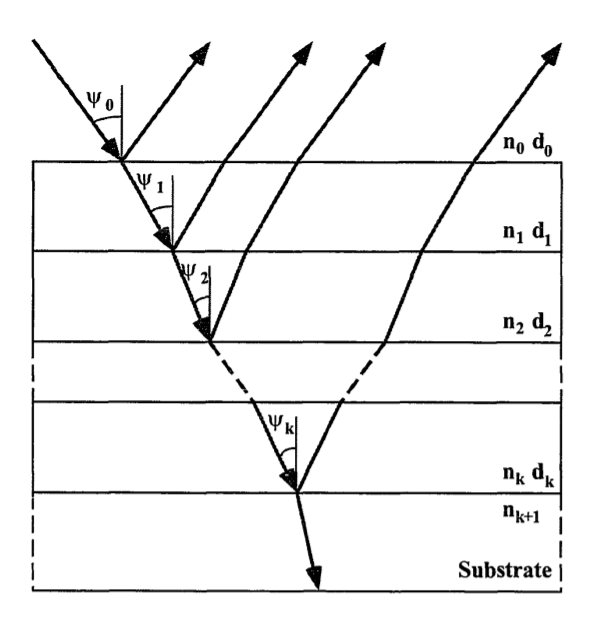
\includegraphics[scale = .8]{Figure 2.6}
	\bf\caption{ Stack of thin film materials.}
	\label{fig:2.6}
\end{figure}

\noindent likewise refers to the electric field traveling up. A similar convention is also adopted for the magnetic field $H$. The following relationship is obtained by solving Maxwell’s equations at each interface [49]


\setstretch{1}
\begin{align}
	\begin{bmatrix} E_{0}^{+} \\ E_{0}^{-} \end{bmatrix} = \frac{(C_{1})(C_{2})...(C_{k+1})}{t_{1}t_{2}...t_{k+1}} \begin{bmatrix} E_{k+1}^{+} \\ E_{k+1}^{-} \end{bmatrix},
\end{align}

\noindent where

\begin{align}
	(C_{m}) = \begin{bmatrix} e^{j\delta_{m-1}} & r_{m}e^{j\delta_{m-1}} \\ r_{m}e^{-j\delta_{m-1}} & e^{-j\delta_{m-1}} \end{bmatrix}.
\end{align}

\noindent We write the matrix product as

\begin{align}
	(C_{1})(C_{2})...(C_{k+1})=\begin{bmatrix} a & b \\ c & d \end{bmatrix}.
\end{align}

\setstretch{1.5}

\noindent If the substrate is thick compared to the absorption wavelength of the incident light, then there is no negative traveling wave at the last interface, i.e., $E_{k+1}^{-} = 0$; thus from Equation 2.16 we obtain


\setstretch{1.5}
\begin{align}
	\frac{E_{0}^{-}}{E_{0}^{+}} = \frac{c}{a}.
\end{align}

\noindent The reflectance $R$ of the multilayer stack is therefore given by [49]

\begin{align}
	R=\frac{\left( E_{0}^{-}\right)\left(E_{0}^{-}\right)^{*}}{\left(E_{0}^{+}\right)\left(E_{0}^{+}\right)^{*}} = \frac{cc^{*}}{aa^{*}}
\end{align}

\setstretch{1.5}
The interference between light reflected from the various surfaces changes as material is removed during the etching process. Therefore, a measurement of the reflectance of the
wafer can be used to determine etch rates during an etch.


\setstretch{1.5}
\noindent\large\bf Reflectometry Hardware

\setstretch{1.5}

\normalsize\normalfont The reflectometry system shown in Figure 2.7 is based on a single wavelength source, provided by a HeNe laser. The beam is modulated by a mechanical chopper before entering

\setstretch{1}
\begin{figure}[H]
	\centering
	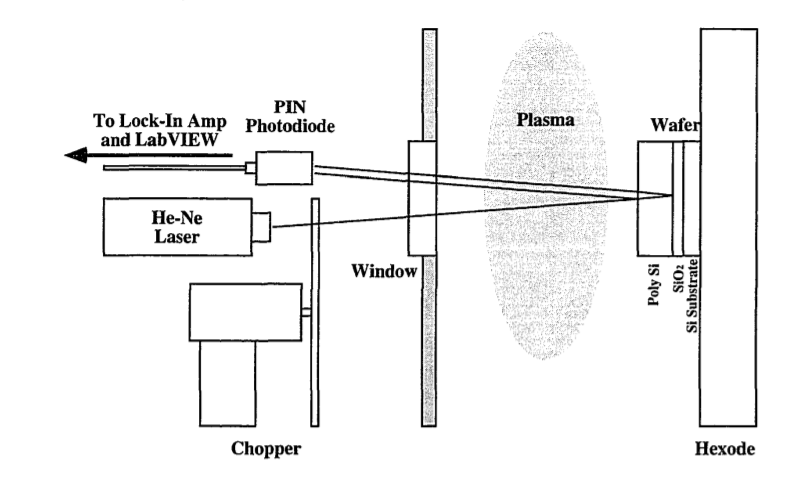
\includegraphics[scale = .7]{Figure 2.7}
	\bf\caption{ Reflectometry system .}
	\label{fig:2.7}
\end{figure}

\setstretch{1.5}

\noindent the chamber. The reflected beam is then collected by a Thorlabs PDA50 p-i-n photodiode and amplified by a Stanford Research SR530 Lock-In Amplifier with a low pass filter time constant of 1 second. This amplifier does not have an automatic phase correction feature,
but this was not a problem as there is ample signal-to-noise in this signal.

A typical trace of the reflectometry signal is shown in Figure 2.8. It can be found
from Equation 2.20 that for a single wavelength of light at normal incidence ($\Psi_{0} = 0$), the peaks and valleys in the interference pattern correspond to thickness differences of
$\frac{1}{4}\frac{\lambda_{0}}{\operatorname{Re}(n)}$ where $\operatorname{Re}(n)$ is the real component of the index of refraction of the layer being etched. For the HeNe wavelength of 632.5 nm, the time between a peak and valley corresponds to the etching of 417$\mathring{A}$ of polysilicon ($\operatorname{Re}(n) = 3.768$). The x’s in Figure 2.9 show the average etch rate (417$\mathring{A}$ divided by the time between the peak and valley) plotted at the midpoint of

\setstretch{1}
\begin{figure}[H]
	\centering
	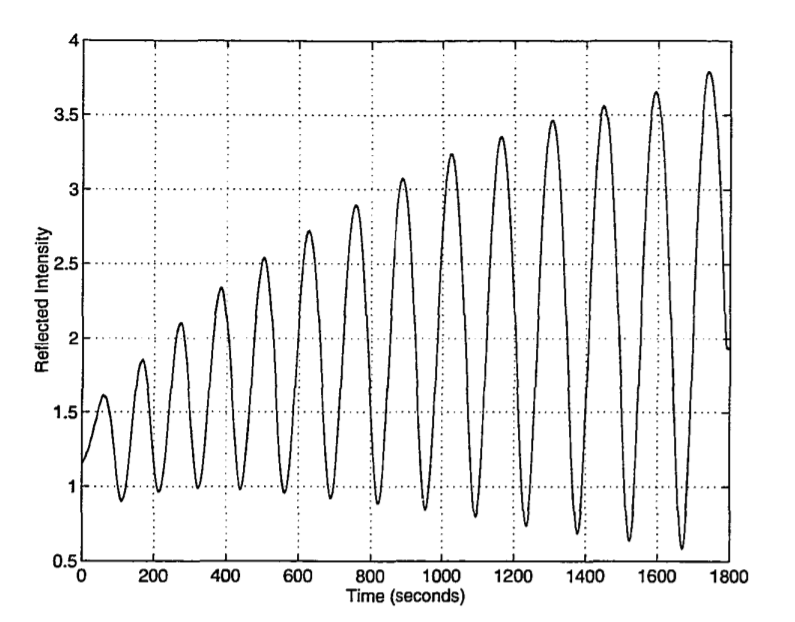
\includegraphics[scale = .55]{Figure 2.8}
	\bf\caption{ Sample reflectometry signal.}
	\label{fig:2.8}
\end{figure}

\setstretch{1.5}
\noindent each time interval. From this figure there appears to be an oscillation in the etch rate, but
this actually is due to the fact that the surface roughness of the polysilicon layer was not
accounted for. To help in visualizing the actual etch rate, a smooth polynomial is fit to this
data as shown in Figure 2.9. Note that data points are only available approximately once
a minute. This is too slow to be used for real-time feedback.

Though not used in this research, two efforts have recently been undertaken to provide
an etch rate measurement for real-time feedback. One of these involves developing an etch
rate estimator which can extract information out of the HeNe signal at a much higher
frequency [104]. The other utilizes a broader band light source, provided by a tungsten
halogen lamp, and a CCD array as a detector [9].


\setstretch{1}
\begin{figure}[H]
	\centering
	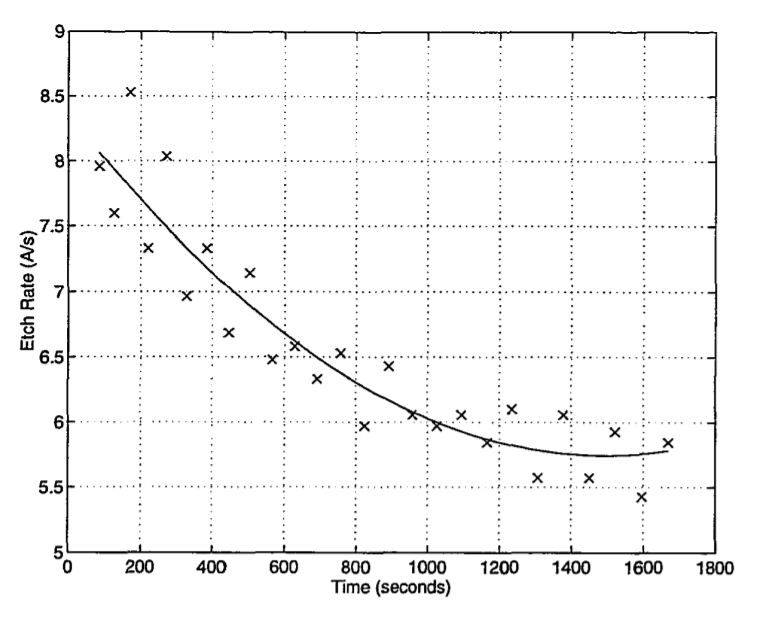
\includegraphics[scale = .55]{Figure 2.9}
	\bf\caption{  Calculated etch rates.}
	\label{fig:2.9}
\end{figure}

\setstretch{1.5}

\section{Data Acquisition and Control Platform}

\tab The largest modification made to the etcher was to upgrade its data acquisition and control software/hardware. Prior to the beginning of this work, the original control system on our AME-8300 had been replaced by a Techware Systems PAL 68000 process control computer. This system was excellent for running event-driven process recipes but was not capable of real-time monitoring and control\footnote{Recently, in joint work with Techware Systems, we have shown that it is possible to implement real-time control algorithms on Techware’s next generation of process control computers, the T-II. Work is continuing to develop a commercially available implementation.}. Two major limitations were: 1) data collection was (asynchronously) polled and 2 ) sampling rates were limited to approximately twice a second. These limitations were overcome by implementing a data acquisition and control system using LabVIEW\footnote{Lab VIEW is a graphics-based programming language from National Instruments that provide drivers for their Interface boards.
} to collect data and perform real-time control actions.


\setstretch{1}
\begin{figure}[H]
	\centering
	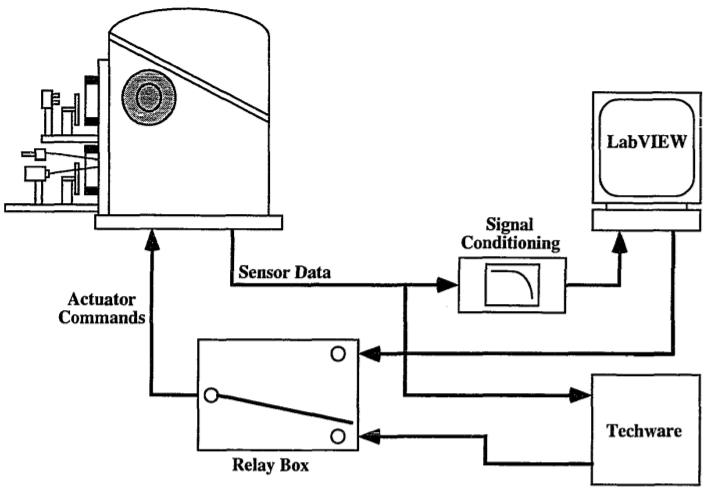
\includegraphics[scale = .55]{Figure 2.10}
	\bf\caption{  Techware and LabVIEW wiring configuration.}
	\label{fig:2.10}
\end{figure}

\setstretch{1.5}

\subsection{LabVIEW Data Acquisition and Control System}

\tab In order to provide the data acquisition and control capabilities necessary to build dynamic models and apply feedback control, an Apple Quadra 950 running LabVIEW was piggy-backed onto the Techware computer. The LabVIEW system was only used during the segment of the etch process when the plasma was lit; wafer loading, pumpdown, venting, etc. are all controlled by the Techware computer. During the time when the plasma is lit, a bank of relays gives control of the equipment setpoints to the LabVIEW system, while sensor data can be simultaneously monitored by both computers. This wiring configuration is shown in Figure 2 .10.


Our LabVIEW system consists of three expansion bus boards:

\noindent\textbf{NB-MIO-16-25L} a multifunction input-output board which has 16 signal-ended 

analog inputs, 2 analog outputs, 8 TTL inputs/outputs, and 3 counter-timers.


\noindent\textbf{NB-AO-6} an analog output board with 6 channels.


\noindent\textbf{NB-DMA-2800} which provided direct memory access (DMA) and a high speed IEEE

488 (GPIB) interface.


In developing the LabVIEW data acquisition and control system, care was taken to synchronize the timing of the various input and output channels. One of the counter/timers (CNTR\#1) was configured to produce a square wave with the period of the sampling interval. This signal is shared among the various boards via a real-time system integration (RTSI) bus, which is a local bus connecting the boards. As seen in Figure 2.11, the sample interval begins on the rising edge of the CNTR\#1 signal. When this rising edge occurs the analog output (AO) channels are updated and reading of the analog input channels (Al) is initiated. While the NB-MIO-16-25L board has 16 input channels, it only has one analog-to-digital (A/D) converter. A multiplexer switches between channels on the rising edge of an AI conversion pulse generated by a second counter (CNTR\#2). The A/D converter on this board has a settling time of 25 $\mu$s; however due to a software bug in the data acquisition drivers the period of the AI conversion pulses was set to 90 $\mu$s. The number of conversions is controlled by CNTR\#1 (the gating pulse), in that the CNTR\#2 only runs when the gating pulse is high. After all of the channels are acquired, the next control action is calculated and the inactive output buffer is loaded with the new values. More details on timing for real-time control implementations can be found in [7].


LabVIEW is a graphics-based programming language in which programs are written by “wiring” icons together. An example of LabVIEW code for reading data from the analog

\setstretch{1}
\begin{figure}[H]
	\centering
	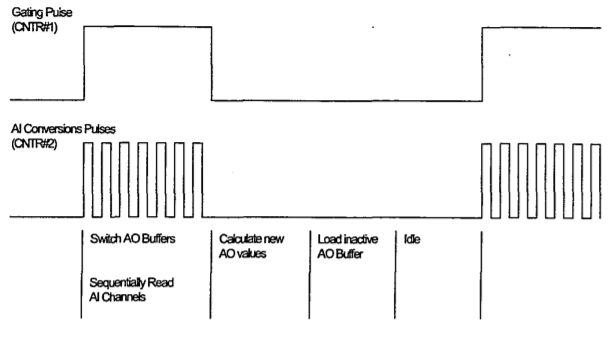
\includegraphics[scale = .65]{Figure 2.11}
	\bf\caption{  Data acquisition timing diagram.}
	\label{fig:2.11}
\end{figure}

\setstretch{1.5}

\noindent input channels is shown in Figure 2.12. LabVIEW also provides the programmer with a number of widgets in which a graphical interface (or panel) can be developed for the user. One such panel is the Control Setup Panel, shown in Figure 2.13. Prom this panel the user can select data acquisition and control parameters for the etch. It allows the user to select the controller file, reference command file and sampling rate to be used for the etch. In addition, the user can select which sensor channels will be displayed to the screen and logged to disk for future analysis. The selected sensor channels are displayed on strip charts on the Monitor Panel (Figure 2.14) during the etch.


\setstretch{1}
\subsection{Signal Preconditioning}
\setstretch{1.5}

In sampling an analog line, it is important to take precautions against a phenomenon known as aliasing [78]. If the signal being sampled contains frequency components that are higher than half the sampling frequency ($f_{s}$) then these components may appear to be low frequency components. This can particularly be a problem if there are high frequency periodic signals [6]. To prevent aliasing, a low-pass filter known as an antialiasing filter is

\setstretch{1}
\begin{figure}[H]
	\centering
	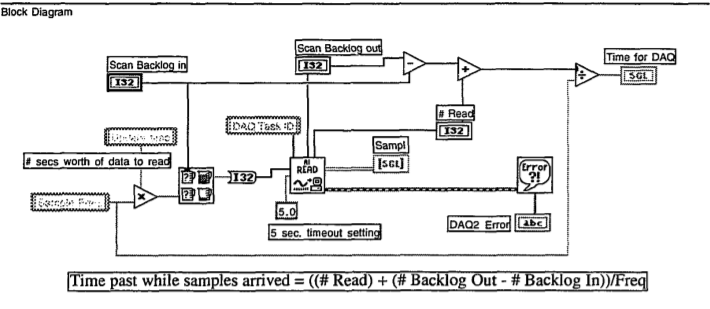
\includegraphics[scale = .7]{Figure 2.12}
	\bf\caption{  Example of LabVIEW code for data acquisition.}
	\label{fig:2.12}
\end{figure}

\setstretch{1}
\begin{figure}[H]
	\centering
	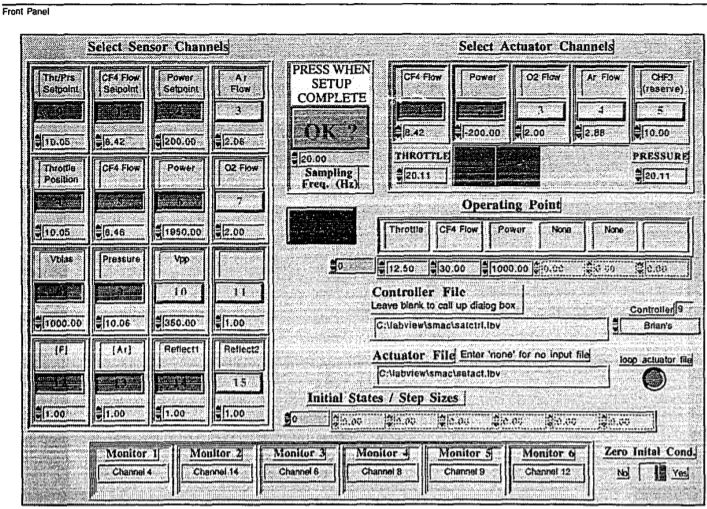
\includegraphics[scale = .7]{Figure 2.13}
	\bf\caption{  LabVIEW Control Setup Panel.}
	\label{fig:2.13}
\end{figure}

\vspace*{3cm}
\setstretch{1.5}
\begin{figure}[H]
	\centering
	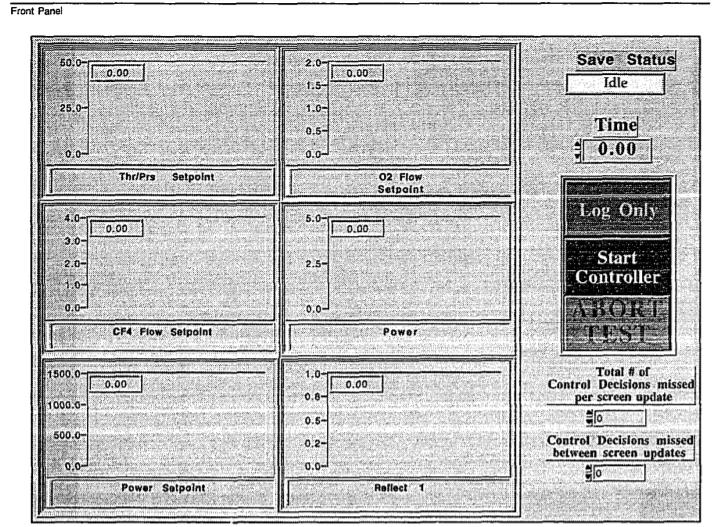
\includegraphics[scale = .8]{Figure 2.14}
	\bf\caption{  LabVIEW Monitor Panel.}
	\label{fig:2.14}
\end{figure}

\newpage

\noindent used to remove high-frequency components from the signals before sampling. Often either Butterworth [78] or Bessel [6] filters are used for this task.

Second-order Butterworth filters were chosen for our system. These were designed around a single operational amplifier as shown in Figure 2.15 [55]. For a Butterworth filter with corner frequency $f_{c}$, the resistors and capacitors are chosen such that


\setstretch{1}
\begin{align}
	f_{c} = \frac{1}{2\pi RC}
\end{align}

\noindent and

\begin{align}
	K=1.586.
\end{align}

\setstretch{1.5}

\noindent The LabVIEW data acquisition system was capable of collecting data at 45 Hz. Therefore, the desired corner frequency was 22.5 Hz. In practice, the resistors and capacitors had to be chosen to correspond to standard values. The filter was implemented with


\setstretch{1}

\begin{align}
	R&=24.1 \text{k}\Omega,\\
	(K-1)R&= 15.9 \text{k}\Omega,
\end{align}

\noindent and

\begin{align}
	C=0.33\mu f.
\end{align}

\noindent These values lead to

\begin{align}
	f_{c}=19.4 \text{Hz}
\end{align}

\noindent and

\begin{align}
	K=1.606.
\end{align}

\begin{figure}[H]
	\centering
	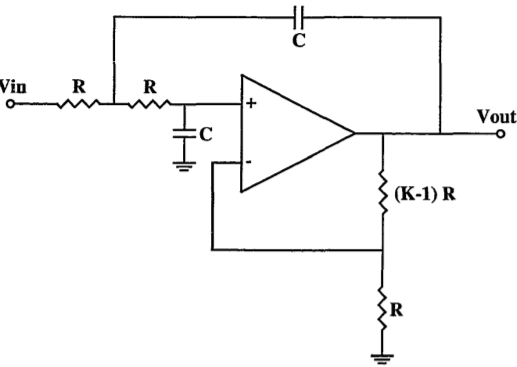
\includegraphics[scale = .7]{Figure 2.15}
	\bf\caption{  Implementation of a lowpass filter.}
	\label{fig:2.15}
\end{figure}

\setstretch{1.5}

The analog input channels on the NB-MIO-16 board were configured with a range of 0 to 10 Volts. If the filters are connected to the input channels at $V_{out}$, the analog channels will saturate at a filter input voltage of $V_{in}$ = 6 V. A voltage divider was added to step the filter gain down to unity. However, because the operational amplifier was powered by ±15 V, $V_{out}$ still saturates at 14.3 V. This saturation occurs at $V_{in}$ = 8.9 V, thus limiting the measurable voltage range to 0 — 8.9 V. In general, this was not a problem for us as most signals remained below 8 volts during normal operation of the system. The exception to this was the optical input signals where it was convenient to have the full 10 volts of range. Recently, the voltage was stepped down at the input stage using a voltage divider and unity gain buffer, as shown in Figure 2.16. This allows the full 0 - 10 V range for the measured inputs. In addition, several of the signals, such as $\text{V}_{bias}$ and power, had ranges between 0 and -10 volts. Therefore, inverting amplifiers were used to bring these voltages into the range of the input channels. Finally, the inverting amplifiers drew enough current on the $\text{V}_{bias}$ channel to actually drop the voltage at the electrode, so a high impedance unity gain buffer was used to isolate the powered electrode from the filter.

\begin{figure}[H]
	\centering
	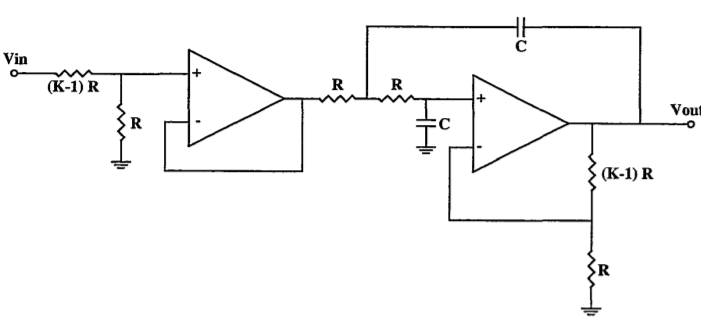
\includegraphics[scale = .7]{Figure 2.16}
	\bf\caption{  Improved lowpass filter.}
	\label{fig:2.16}
\end{figure}